

\paragraph*{Status, 25 October 2026 (Part 2).} This chapter adds to Part 1 the thermal premise: a static metric, a normalized Killing time, the Hawking conversion and the quarter-area entry convention (register T-13). The finite-entry staircase and its Catalan series are exact conditional mathematics; the entry convention is declared, not derived. One run touches it: volii\_gate\_1 (ironclad H002782), whose reading is that a step temperature named from a hazard is a change of name (Arrhenius through the saddle, $T_A\to 1/\beta$), not an identification.


\section{Purpose, premises, and the boundary question}
The unit-accumulation surface joins three subjects that must remain logically distinct: exterior geometry, thermodynamic bookkeeping, and accessible information. Chapter V supplies a static exterior adapter and an exact finite ledger. Chapter VI supplies the operational meaning of a record and the contraction of distinguishability under restricted access. This chapter assembles those results, extends their elementary consequences, and identifies the additional physical input needed for an absolute radiation law.

The principal outcome is conditional but precise. Given the Schwarzschild exterior adapter, the usual normalization of time at infinity, the Hawking temperature conversion, and the retained quarter-area entropy rule, the horizon temperature and differential first law agree with semiclassical black-hole thermodynamics. Given the integer-entry continuation, the exact energy of a finite emission follows algebraically. Neither statement derives the adapter, the quarter-area rule, or an emission clock from the microscopic source. Keeping these dependencies visible prevents an agreement inherited from an input from being counted a second time as an independent prediction.

The finite Si29 example provides a different kind of result. Its reported relative-entropy Hessian is not proportional to its enclosing-area Hessian, and entropy together with area locally distinguishes two source directions. This is a useful obstruction to a particular finite-source information map. It is not a disproof of a continuum horizon identity formulated for a different area, state family, and perturbation order.

Throughout this chapter, $A(r)$ denotes dimensionless accumulation, $\mathcal A_H$ denotes physical horizon area, and $N$ denotes the dimensionless entropy-entry count. These are different objects. In particular, $A(r_H)=1$ does not mean that the physical area is one square metre or one Planck area. Entropies written as $s$ are dimensionless, with physical entropy $S=k_Bs$. This convention keeps logarithmic quantum-information expressions separate from thermodynamic units.

\subsection{Evidence levels}
Four levels of statement recur. An \emph{input} is an adopted bridge or constitutive premise. A \emph{conditional derivation} follows from such inputs by explicit mathematics. A \emph{retained calculation} is reported in the supplied source record but has not been rerun here. An \emph{open closure} is a missing physical map, experiment, or computation. The expanded calculations below are analytic consequences of printed premises; they are not new native source runs.

The closure surface also requires a causal interpretation. The divergence of a static coordinate travel time does not by itself prove that an infaller cannot cross a regular horizon. In the adopted metric, radial free-fall trajectories can reach the horizon in finite proper time. SAM's rule about completion of the parent ledger therefore needs its own operational statement: which event, record, or custody transfer is forbidden, and with respect to which observer? A restriction on exterior record access is weaker than a reflecting material wall. The distinction will matter both for radiation and for observational limits on compact surfaces.

\section{Surface gravity from a specified exterior}
\subsection{Three gradients, three different meanings}
Consider the static, spherically symmetric line element
\begin{equation}
 ds^2=-F(r)c^2dt^2+H(r)dr^2+r^2d\Omega^2,
 \qquad F>0,\quad H>0,
 \label{c7:metric}
\end{equation}
with Killing time normalized so that $F\to1$ at infinity. Chapter V adopts
\begin{equation}
 A(r)=\frac{r_s}{r},\qquad r_s=\frac{2GM}{c^2},\qquad
 F=1-A,\qquad H=F^{-1}.
 \label{c7:adapter}
\end{equation}
The areal-coordinate derivative $|A'|=r_s/r^2$ tends to $1/r_s$. The spatial proper gradient on a static slice is $|A'|/\sqrt H$, which tends to zero. Neither quantity alone is the surface gravity. Surface gravity is the redshifted acceleration required to hold a static observer near the horizon, with a specified normalization of the time-translation generator.

A static worldline has $d\tau=\sqrt F\,dt$. Evaluating its four-acceleration gives the positive magnitude
\begin{equation}
 a_{\rm stat}=\frac{c^2|F'|}{2F\sqrt H},\qquad
 \kappa=\lim_{r\downarrow r_s}\sqrt F\,a_{\rm stat}
       =\frac{c^2}{2}\lim_{r\downarrow r_s}\frac{|F'|}{\sqrt{FH}}.
 \label{c7:acceleration}
\end{equation}
The first denominator contains $F\sqrt H$, not merely $\sqrt{FH}$. This distinction separates local proper acceleration, which diverges for the adopted adapter, from its finite redshifted limit. Substituting $FH=1$ yields
\begin{equation}
 \kappa=\frac{c^2}{2r_s}=\frac{c^4}{4GM}.
 \label{c7:kappa}
\end{equation}
The normalization of $r_s$ is inherited from the earlier gravitational bridge; the result also uses the spatial metric adapter. A scalar inverse-radius kernel without a spatial metric does not establish this surface gravity.

The temperature conversion of semiclassical horizon theory is
\begin{equation}
 T_H=\frac{\hbar\kappa}{2\pi ck_B}
     =\frac{\hbar c^3}{8\pi GMk_B}.
 \label{c7:temperature}
\end{equation}
Hawking's field-theoretic calculation supplies this conversion [VII.1]. Here it is used as a bridge rather than rederived from the finite substrate source. For one solar mass the retained example gives $r_s\simeq2.953\,\mathrm{km}$, $\kappa\simeq1.522\times10^{13}\,\mathrm{m\,s^{-2}}$, and $T_H\simeq6.17\times10^{-8}\,\mathrm K$. The scaling with mass is more robust than the final displayed digits: $r_s\propto M$, while $\kappa$ and $T_H$ are proportional to $M^{-1}$.

\subsection{Local temperature and equilibrium}
If a stationary thermal state is in equilibrium with respect to the same Killing time, the locally measured temperature obeys the Tolman redshift relation
\begin{equation}
 T_{\rm loc}(r)\sqrt{F(r)}=T_\infty.
 \label{c7:tolman}
\end{equation}
One way to see the relation is to require the same occupation factor for a quantum described locally or at infinity. Since $E_\infty=\sqrt F E_{\rm loc}$, equality of $E/(k_BT)$ gives equation~\eqref{c7:tolman}. This derivation establishes a consistency condition on equilibrium descriptions; it does not say that an arbitrarily accelerated detector or a freely falling detector measures the same temperature.

The divergence of $T_{\rm loc}$ as $F\to0$ belongs to an ideal family of static observers whose required acceleration also diverges. It must not be interpreted as a measured infinite temperature on a freely falling material thermometer. A real static apparatus has finite strength, finite size, and a backreaction that invalidates the ideal limit. This observer dependence is especially important if the parent-ledger language is later attached to detector records.

\section{Entropy entries and the first law}
\subsection{Coefficient provenance}
Set $\ell_P^2=\hbar G/c^3$. The retained four-cell entry convention reads
\begin{equation}
 \mathcal A_H=4\pi r_s^2,\qquad
 N=\frac{\mathcal A_H}{4\ell_P^2}
   =\frac{4\pi GM^2}{\hbar c},\qquad
 S_H=k_BN.
 \label{c7:entropy}
\end{equation}
The area law is the Bekenstein--Hawking normalization [VII.1--VII.2], adopted here as the retained area-entry premise. The fact that an entry is called four-cell does not independently prove that its microscopic degeneracy has logarithm one. Those are separate physical claims until the counting measure and state space are specified.

Differentiating equation~\eqref{c7:entropy} gives
\begin{equation}
 dS_H=\frac{8\pi GMk_B}{\hbar c}\,dM,
 \qquad T_HdS_H=c^2dM.
 \label{c7:firstlaw}
\end{equation}
Thus the adopted temperature and entropy laws are mutually consistent with the first law for a neutral, nonrotating, quasistatic family. Angular momentum, charge, exterior work, and matter fluxes are absent from this restricted calculation. Their thermodynamic potentials cannot be obtained by relabelling $M$ in this expression.

\begin{center}
\small
\begin{tabularx}{\linewidth}{@{}lXX@{}}
\toprule
Coefficient & Place in calculation & Logical source\\
\midrule
$2$ & $r_s=2GM/c^2$ & Earlier gravitational normalization\\
$1/2$ & Redshifted acceleration & Metric adapter and static observer\\
$1/(2\pi)$ & $T_H=\hbar\kappa/(2\pi ck_B)$ & Semiclassical temperature bridge\\
$1/4$ & $N=\mathcal A_H/(4\ell_P^2)$ & Retained entropy-entry premise\\
$k_B$ & Entropy per entry & Retained thermodynamic convention\\
\bottomrule
\end{tabularx}
\end{center}
Each coefficient has one place in the argument. Agreement of the final expression does not erase the need to derive the bridges if a microscopic explanation is claimed.

The heat capacity along this family is negative:
\begin{equation}
 C_H=\frac{d(Mc^2)}{dT_H}
 =-\frac{Mc^2}{T_H}=-2k_BN.
 \label{c7:heatcapacity}
\end{equation}
This follows because decreasing mass raises the temperature. It warns against treating an isolated finite reservoir as a stable canonical bath of unlimited capacity. The finite-entry construction is particularly useful because it does not require that approximation.

\subsection{What is, and is not, an integer count}
Equation~\eqref{c7:entropy} assigns a real number $N$ to every positive mass. The additional statement that allowed states lie on integer $N$ is a quantization hypothesis. On that hypothesis,
\begin{equation}
 M_N=\sqrt{\frac{\hbar c}{4\pi G}}\sqrt N,
 \qquad E_N=\sqrt{\frac{\hbar c^5}{4\pi G}}\sqrt N.
 \label{c7:levels}
\end{equation}
The mathematical sequence exists for $N=0,1,2,\ldots$. Its applicability to Planck-scale endpoints is not established by a semiclassical temperature law. In particular, a formation floor or remnant condition from Chapter XII may restrict the admissible sequence to $N\ge N_{\rm floor}$ and remove some terminal transitions entirely.

There is also a microscopic counting subtlety. If $S_H=k_B\log g_N=k_BN$ were an exact entropy of uniformly weighted, finite microcanonical states, it would imply $g_N=e^N$, which is not an integer for positive integer $N$. Consequently the entry entropy cannot simultaneously be interpreted as an exact logarithm of a finite integer degeneracy with that literal normalization, unless further structure changes the interpretation. It can instead be a thermodynamic entropy, an effective shell weight, or an asymptotic count. The chapter's conditional balance formulas use such weights; they do not supply the missing integer degeneracy. This distinction also matters when comparing alternative discrete-area proposals.

\section{Exact finite transitions}
\subsection{One-entry emission}
For an allowed transition from $N$ to $N-1$, take the emitted energy positive and write $\Delta S_{\rm loss}=k_B$. The horizon's signed entropy change is $-k_B$. Direct subtraction of equation~\eqref{c7:levels} gives
\begin{equation}
 \Delta E=Mc^2\left(1-\sqrt{1-\frac1N}\right),\qquad
 \frac{\Delta E}{k_BT_H(M)}
 =\frac{2}{1+\sqrt{1-1/N}}.
 \label{c7:onestep}
\end{equation}
The rationalized form avoids numerical cancellation at large $N$. It also proves immediately that the ratio lies in $[1,2]$, approaches one at large $N$, and equals two at $N=1$. These statements are exact properties of the assumed sequence, not a measured endpoint spectrum.

Let $q=1/N$ and $c_*(q)=\Delta E/(k_BT_H)$. Multiplication by the conjugate, followed by rearrangement, gives
\begin{equation}
 c_*=1+\frac q4c_*^2,
 \qquad c_*(q)=\sum_{j=0}^{\infty}\frac{C_j}{4^j}q^j,
 \qquad C_j=\frac{1}{j+1}\binom{2j}{j}.
 \label{c7:catalan}
\end{equation}
The branch satisfying $c_*(0)=1$ is selected. The first terms are $1+q/4+q^2/8+5q^3/64+\cdots$. Since $0<C_j/4^j\le1$, for $0\le q<1$ the remainder after degree $m$ obeys
\begin{equation}
 0\le c_*(q)-\sum_{j=0}^{m}\frac{C_j}{4^j}q^j
 \le\frac{q^{m+1}}{1-q}.
 \label{c7:remainder}
\end{equation}
This is a deliberately simple bound rather than an optimal one. It is uniform on every interval $0\le q\le q_0<1$ and provides a reproducible error estimate for the large-ledger approximation.

The ratios at $N=1,2,10,100$ are respectively $2$, $1.17157$, $1.02633$, and $1.00251$. The solar-mass example has approximately $1.05\times10^{77}$ entries, so its correction is of order $10^{-78}$. The finite law therefore has mathematical endpoint content while giving no practical temperature correction for a stellar-mass hole.

\subsection{Multiple entries and a finite first law}
For $0<j\le N$ the same calculation gives
\begin{equation}
 \begin{aligned}
 \Delta E_j&=Mc^2\left(1-\sqrt{1-j/N}\right),\\
 \frac{\Delta E_j}{k_BT_H(M)}
 &=\frac{2j}{1+\sqrt{1-j/N}}
\\&=j+\frac{j^2}{N(1+\sqrt{1-j/N})^2}.
 \end{aligned}
 \label{c7:jstep}
\end{equation}
The initial temperature underestimates the energy per unit entropy lost because the reservoir heats while it loses mass. The exact finite first law is an integral,
\begin{equation}
 \Delta E_j=\int_{N-j}^{N}k_BT_H(n)\,dn,
 \qquad T_{\rm step}=\frac{\Delta E_j}{jk_B}.
 \label{c7:step-temperature}
\end{equation}
For $j<N$, monotonicity gives $T_H(N)\le T_{\rm step}\le T_H(N-j)$. At the endpoint the upper limit diverges in the extrapolated temperature formula, but the integral stays finite. Defining a step temperature in this manner is an exact thermodynamic average, not an independent thermometer prescription.

This distinction clarifies the retained phrase ``the final entry carries twice its thermal energy.'' It means twice $k_BT_H$ evaluated at the initial level $N=1$. It does not mean twice the temperature of a nonexistent final black hole, and it does not by itself specify the number of particles sharing that energy. One ledger transition could distribute its energy among multiple coupled channels if the source dynamics allows it.

\section{Detailed balance and its assumptions}
Suppose initial and final microcanonical shells have effective weights proportional to $e^{S_H/k_B}$, and suppose the emission and reversed absorption channels have matched dynamical matrix elements and compatible measures. Then the ratio of shell-averaged transition weights is
\begin{equation}
 \frac{\Gamma_{\rm em}}{\Gamma_{\rm abs}}
 =\exp\left[\frac{S_H(E-\varepsilon)-S_H(E)}{k_B}\right].
 \label{c7:balance}
\end{equation}
For an allowed $j$-entry transition the exponent is exactly $-j$. This proves the conditional ratio $e^{-j}$ under the stated channel and counting assumptions. It does not prove equality of unmatched scattering channels, equal matrix elements for all transitions, or a total emission rate.

Writing $S_H(E)/k_B=aE^2$ with $a=4\pi G/(\hbar c^5)$ makes finite backreaction transparent:
\begin{equation}
 \frac{\Delta S_H}{k_B}=-2aE\varepsilon+a\varepsilon^2
 =-\frac{\varepsilon}{k_BT_H(E)}+a\varepsilon^2.
 \label{c7:backreaction}
\end{equation}
The correction is positive relative to a fixed-initial-temperature Boltzmann exponent. Its sign is another expression of negative heat capacity. Evaluated on the discrete energy gaps, the entire exponent remains $-j$; one must not apply the $e^{-j}$ factor and then add this backreaction a second time.

For a finite ladder $\varepsilon_n=n\varepsilon_Q$, $0\le n\le K$, the correction to the log weight lies in an interval of width $a(K\varepsilon_Q)^2$. A standard bounded-likelihood-ratio argument gives the retained total-variation estimate
\begin{equation}
 \|p_{\rm back}-p_{\rm fixed}\|_{\rm TV}
 \le\tanh\!\left[\frac{a(K\varepsilon_Q)^2}{4}\right].
 \label{c7:tvback}
\end{equation}
Indeed, reweighting a probability law by $e^f$ with $\max f-\min f=L$ has extremal variation bounded by $\tanh(L/4)$; the extremum is obtained by concentrating weight at the endpoints and optimizing their initial probabilities. The bound requires that the same finite support and channel measure are used on both sides. It is not a claim about arbitrary changes of species, boundary state, or detector acceptance.

\begin{figure*}[t]
\centering
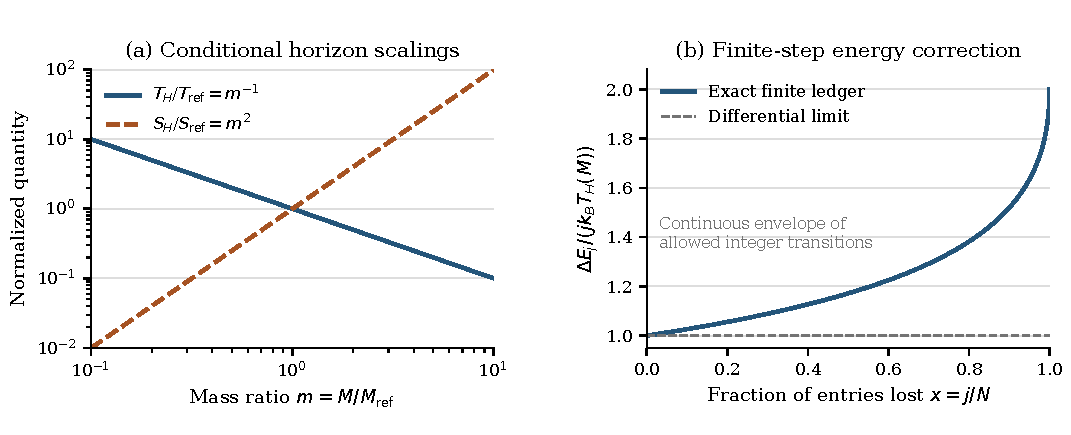
\includegraphics[width=\textwidth]{figures/ch07_horizon_scalings.pdf}
\caption{Conditional horizon thermodynamics and the finite ledger. (a) The adopted Schwarzschild geometry, Hawking temperature conversion and quarter-area entropy rule give $T_H/T_{\rm ref}=(M/M_{\rm ref})^{-1}$ and $S_H/S_{\rm ref}=(M/M_{\rm ref})^2$, with both reference quantities evaluated at $M_{\rm ref}$. (b) The exact entry ledger gives $\Delta E_j/(jk_BT_H)=2/[1+\sqrt{1-j/N}]$. The continuous curve is an envelope of integer transitions; its value at zero is the differential limit. Extension to complete entry loss is conditional and need not be physically allowed by a formation floor. These analytic curves are neither an emission spectrum nor a newly simulated source result.}
\label{fig:c7:scalings}
\end{figure*}

\section{From finite occupations to transmitted counts}
\subsection{The truncated geometric law}
The retained HOME-QW1 occupation law has
\begin{equation}
 p_n=\frac{q^n}{Z_K},\quad 0\le n\le K,\qquad
 Z_K=\frac{1-q^{K+1}}{1-q},\qquad 0<q<1.
 \label{c7:geometric}
\end{equation}
Its exact mean follows by differentiating $\log Z_K$:
\begin{equation}
 \langle n\rangle_K=q\frac{d}{dq}\log Z_K
 =\frac{q}{1-q}-\frac{(K+1)q^{K+1}}{1-q^{K+1}}.
 \label{c7:mean}
\end{equation}
The infinite law is $(1-q)q^n$. The finite law is that law conditioned on $n\le K$, so their total-variation distance equals the omitted probability $q^{K+1}$. This elementary proof supplies a transparent finite-capacity error criterion: choose $K$ such that $q^{K+1}$ is below the required tolerance. It is not enough merely to say that $K$ is large, because convergence is slow when $q$ is close to one.

An occupation distribution specifies diagonal number statistics but not the complete density operator. States with the same probabilities can differ in phase coherence, inter-guide correlations, and entanglement with the retained reservoir. For a thermal interpretation the basis, Hamiltonian, and state preparation must all be named. In particular, the model relation $q=e^{-\omega/T_A}$ uses source units. Converting it into $e^{-\hbar\omega_{\rm phys}/k_BT_H}$ requires the energy and clock bridge discussed below.

\subsection{Transmission and noise}
Chapter V reports the annular Jost transmission
\begin{equation}
 \tau_{\rm eff}(k)=\frac{4k^2}{|D(k)|^2},\qquad
 0<\tau_{\rm eff}\le1,
 \label{c7:jost}
\end{equation}
for its specified real, passive scattering problem and positive open-channel wave number. Wronskian conservation establishes flux conservation in that problem. A different dissipative boundary, coupled species, or unequal asymptotic channel velocities would require a corresponding flux normalization and scattering calculation. The retained formula is therefore a result for its stated annulus, not automatically every black-hole greybody factor.

For a number state entering a passive loss channel with the other input in vacuum, transmitted counts obey
\begin{equation}
 P(m\mid n)=\binom nm\eta_f^m(1-\eta_f)^{n-m}.
 \label{c7:binomial}
\end{equation}
Here $\eta_f$ is the transmission and detection efficiency for the selected wave packet. For an input mixture, the law of total expectation and variance yields
\begin{align}
 \langle m\rangle&=\eta_f\langle n\rangle,\label{c7:countmean}\\
 \operatorname{Var}(m)&=\eta_f(1-\eta_f)\langle n\rangle
                 +\eta_f^2\operatorname{Var}(n).\label{c7:countvar}
\end{align}
Thus transmission changes both the mean and counting noise. These equations provide a stronger check than mean flux alone. They cease to be the complete answer when the unused port is populated or correlated with the incident mode; in that case interference and stimulated contributions must be retained.

The stationary two-guide convention retained in Chapter V gives $d\dot N/d\omega=\tau_{\rm eff}n_A/\pi$. The factor $1/\pi$ belongs to that channel normalization and population choice. A physical mode sum is often organized instead as
\begin{equation}
 L_\infty=\sum_{s,\ell,m}\int_0^\infty\frac{d\omega}{2\pi}
 \hbar\omega\,\Gamma_{s\ell m}(\omega)\,n_{s\ell m}(\omega),
 \label{c7:luminosity}
\end{equation}
with the channel measure and degeneracies explicitly stated. Equation~\eqref{c7:luminosity} is a template, not a newly computed SAM luminosity. It demonstrates exactly where the source state, energy conversion, species content, and transmission must meet.

\section{Area and information in Si29}
\subsection{Relative entropy has no linear term}
For a faithful finite reference state $\sigma$, define $K_\sigma=-\log\sigma$ and
\begin{equation}
 \begin{aligned}
 D(\rho\Vert\sigma)&=\operatorname{Tr}\rho(\log\rho-\log\sigma)\\
 &=\Delta\langle K_\sigma\rangle-\Delta s_{\rm vN},\\
 s_{\rm vN}&=-\operatorname{Tr}\rho\log\rho.
 \end{aligned}
 \label{c7:relative}
\end{equation}
Take a smooth normalized family $\rho(x)$ with $\rho(0)=\sigma$. Its entropy differential at the reference is $ds_{\rm vN}=\operatorname{Tr}(d\rho K_\sigma)$, since $\operatorname{Tr}d\rho=0$. Hence $dD=0$. Relative entropy is stationary at its reference for general structural reasons. If an area observable has a nonzero first derivative, a proposed equality $\Delta\overline{\mathcal A}=cD$ fails immediately along that direction.

That observation is generic. It does not test a continuum identity in which both flux and area response are quadratic in an excitation amplitude. Dorau and Much analyze coherent excitations and horizon energy flux under an entropy-area assumption [VII.4]. Their geometrical area is not automatically the finite-source enclosing area. A valid comparison must align the state family, reference, perturbation parameter, geometric map, and order before comparing coefficients. This is the required correction to the earlier first-order interpretation.

\subsection{The substantive Hessian comparison}
The retained Si29 record uses a four-by-eighteen tensor source, seed $(3,10)$, the original $Q/G$ matrices, reference phases $0.007$ and $0.013$, and two perturbations $x=(u,v)$. Its common-energy enclosing area is $\overline{\mathcal A}=\mathcal A/(4\pi a^2)$ at $e=4$. The record reports 34 signed perturbations and the exact decomposition~\eqref{c7:relative}. Numerical matrices quoted here are its rounded reported results, not new interval certificates.

With $G$ the relative-entropy Hessian and $H_{\mathcal A}$ the area Hessian, the two references give
\begin{align}
 G_{.007}&=\begin{pmatrix}252.754&-785.399\\-785.399&17867.308\end{pmatrix},\\
 H_{.007}&=\begin{pmatrix}7.753&-6.015\\-6.015&445.393\end{pmatrix},\label{c7:hess1}\\
 G_{.013}&=\begin{pmatrix}110.500&-516.332\\-516.332&7083.046\end{pmatrix},\\
 H_{.013}&=\begin{pmatrix}4.095&-11.510\\-11.510&-24.842\end{pmatrix}.
 \label{c7:hess2}
\end{align}
At the first reference, the ratios of corresponding diagonal entries already disagree. At the second reference, $G$ is positive definite while $H_{\mathcal A}$ is indefinite: its diagonal entries have opposite signs. No real scalar multiple of a positive-definite matrix is indefinite. Therefore the quadratic forms are not proportional at either reference.

For a strict second-order test, subtract the linear area variation and compare
\begin{equation}
 \overline{\mathcal A}(x)-\overline{\mathcal A}(0)
 -\nabla\overline{\mathcal A}(0)\cdot x
 =\tfrac12x^TH_{\mathcal A}x+O(\|x\|^3)
\end{equation}
with $D=\tfrac12x^TGx+O(\|x\|^3)$. This is a coordinate-explicit statement about the chosen finite family. A physical horizon map could contain extra terms or different observables; the present calculation constrains such a map but does not exclude all possible maps.

\subsection{Two observables and a local inverse}
The retained local phase direction preserves entropy, whereas the interaction phase changes the reduced spectrum. Setting $y=(s_{\rm vN},\overline{\mathcal A})$ gives
\begin{equation}
 J=\frac{\partial y}{\partial x}
 =\begin{pmatrix}0&s_v\\ \overline{\mathcal A}_u&\overline{\mathcal A}_v\end{pmatrix},
 \qquad \det J=-s_v\overline{\mathcal A}_u.
 \label{c7:jacobian}
\end{equation}
The source reports determinant enclosures excluding zero, with magnitudes about $3.3636$ and $3.5531$. If the reported differentiability and enclosure hypotheses hold, the inverse-function theorem establishes an open neighborhood on which these two observables are valid local coordinates. It does not establish global uniqueness, cover periodic phase identifications, or reconstruct all states in the full tensor space.

The reported inverse errors decrease by approximately four when the grid step is halved: from $7.88\times10^{-5}$ to $1.97\times10^{-5}$ at the first reference, and from $1.02\times10^{-5}$ to $2.56\times10^{-6}$ at the second. This supports second-order local behavior on that sample. A certified neighborhood still needs uniform derivative bounds. One sufficient criterion is
\begin{equation}
 \sup_{x\in B_r}\|J(0)^{-1}[J(x)-J(0)]\|<1,
 \label{c7:inversecriterion}
\end{equation}
on a convex ball $B_r$. It controls departure from the invertible linear map and gives an injectivity estimate there. Selecting $r$ requires native bounds not printed in the present source.

Because $\nabla D=0$ at the reference, its Hessian transforms as a metric under this coordinate change:
\begin{equation}
 G_y=J^{-T}GJ^{-1},\qquad
 g_{tt}=w^TGw,\qquad w=(1+8\nu_{\rm Si},\nu_{\rm Si}).
 \label{c7:metrictransport}
\end{equation}
No extra Hessian-of-coordinate term survives when the gradient vanishes. Mixed entries are expected and encode joint sensitivity; discarding them would lose information. The tangent $w$ belongs to the retained tensor dynamics. Its use as a physical time response still needs a time calibration and a boundary coupling.

\section{Accessible records and boundary custody}
For a completely positive trace-preserving access channel $\mathcal E$, trace distance contracts:
\begin{equation}
 \tfrac12\|\mathcal E(\rho_0)-\mathcal E(\rho_1)\|_1
 \le\tfrac12\|\rho_0-\rho_1\|_1.
 \label{c7:contraction}
\end{equation}
This is the operational content of Chapter VI's accessibility result. A receiver with restricted access cannot distinguish two alternatives better than a receiver supplied with the full state. It is a statement about obtainable records, not a proof that inaccessible global alternatives cease to exist. Conversely, postselected conditioning is not generally a trace-preserving map, so its apparent amplification of distinguishability must include the success flag and its probability.

The boundary pair-write proposes an outward and inward alternative while they are unresolved. The outward member may become an exterior record through allowed transmission and reception. The inward member is unavailable to that exterior observer under the proposed causal cut. Born weighting assigns probabilities once the state and measurement are defined. Neither the accessibility theorem nor the word ``pair'' fixes a pair-production Hamiltonian, a pair rate, or an entanglement spectrum.

The completed-Home custody laws retained from H000794--H000797 add constraints: failed inward transfers return their receipts unchanged; retained exterior receipts have finite inward/outward schedules ending in a parent-side mass-loss event; gross emission and net growth can coexist; and formation mass and radius provide a floor. These are lifecycle commitments to be reconciled with the admissible transitions. If $N_{\rm floor}>0$, the terminal $N=1\to0$ extrapolation cannot be advertised as a realized decay without an additional rule explaining how it avoids the floor.

A useful correlation test would specify joint observables and compare the full outgoing state with a mixture having identical one-mode occupations. Equal Planck-like marginals do not imply equal mutual information or equal conditional records. The target should therefore be a connected correlation, a channel-resolved covariance, or a recovery fidelity with an explicit reference system. At present these are defined measurement opportunities, not computed predictions of the retained occupation law.

\section{A horizon is not automatically a material surface}
A no-completed-crossing statement admits several mathematical implementations. A purely causal horizon can absorb exterior perturbations into degrees of freedom inaccessible to exterior receivers. A timelike surface can reflect, absorb and later re-emit, or store energy. These possibilities have different Green functions and observational consequences. A boundary condition must specify which implementation is intended.

For a radial mode near a boundary in tortoise coordinate $r_*$, write schematically
\begin{equation}
 \psi\sim e^{-i\omega r_*}+\mathcal R(\omega)e^{+i\omega r_*}.
 \label{c7:reflection}
\end{equation}
An ingoing horizon condition has $\mathcal R=0$ in the appropriate classical exterior problem. A reflecting wall has nonzero $\mathcal R$. An absorbing response requires a causal, passive frequency-dependent impedance or additional open channels. This is a parametrization of the missing boundary law, not a new fitted SAM coefficient. The two-polarization source must select the response before either greybody transmission or Chapter XI's ringdown poles can be called native predictions.

Visible surfaces are constrained by accretion energetics. Broderick, Loeb, and Narayan's Sgr A* analysis combines compactness and infrared limits to constrain thermalized surface emission [VII.5]. Its quoted bound places putative visible emission below $0.4\%$ of the accretion luminosity under that analysis's stationary assumptions. This is relevant to a material surface that retains and reradiates accretion energy; it is not a universal exclusion of every causal boundary model. SAM must state its thermalization efficiency, storage time, escape probability, and outflow budget before applying such a bound. Invoking redshift alone does not close the energy account.

\section{Energy conservation, entropy balance, and the missing evolution law}
A radiation model must distinguish instantaneous power from the entropy carried by that radiation. For a parent whose exterior mass is $M(t)$, an idealized energy balance in the infinity-normalized clock is
\begin{equation}
 c^2\frac{dM}{dt}=P_{\rm in}-L_\infty-P_{\rm other}.
 \label{c7:massbalance}
\end{equation}
Here all fluxes refer to the same energy normalization and boundary of the account. $P_{\rm other}$ denotes explicitly modeled outward channels not included in the radiation luminosity. It must not serve as an unconstrained sink inserted to repair disagreement. If energy is stored temporarily in exterior fields or a boundary reservoir, its time derivative belongs on the left or in a separately tracked equation. An emission event can therefore coexist with net growth when inward power is larger than total outward power, exactly as the retained custody language allows.

For slowly evolving neutral configurations, the instantaneous first law gives
\begin{equation}
 \dot S_H=\frac{c^2\dot M}{T_H}.
 \label{c7:entropyrate}
\end{equation}
This is not the total entropy-production law. Exterior matter, radiation, and correlations also contribute. A generalized-entropy candidate has the form $S_{\rm gen}=S_H+S_{\rm outside}$, with a declared subtraction or regulator if continuum field entanglement is involved. The sign of $\dot S_{\rm gen}$ cannot be read off from $\dot S_H$ alone. During emission $S_H$ decreases, while the exterior entropy and correlations may increase. Proving a nondecreasing generalized entropy requires dynamics and a state, not merely the area coefficient.

The same point appears in a single finite transition. Knowing that the horizon loses $jk_B$ of thermodynamic entropy does not imply that a measured photon string carries exactly $jk_B$ of Shannon entropy. The record may be conditioned on detection, share correlations with other channels, or have an entropy dependent on coarse graining. An explicit channel state would allow the von Neumann entropy before and after the interaction to be computed with compatible subsystem definitions. Without it, identifying entropy loss with accessible information is an additional hypothesis.

A minimal dynamical completion could be expressed through populations $P_N(t)$ and rates $W_{N\to N-j}$:
\begin{equation}
 \dot P_N=\sum_j\bigl[P_{N+j}W_{N+j\to N}
                    -P_NW_{N\to N-j}\bigr]
 \label{c7:master}
\end{equation}
for a purely emitting process, with absorption terms added when relevant. The boundary conditions on this equation must enforce normalization, positivity, and any formation floor. The energy expectation then evolves as $\sum_N E_N\dot P_N$, which must equal the integrated outgoing flux computed from the same transitions. This provides a direct conservation test joining the ledger and the spectrum.

Equation~\eqref{c7:master} is a specification of what a completion must supply; no rates have been inferred here. Detailed balance constrains ratios of forward and reverse rates in a suitable equilibrium setting, whereas multiplication of every rate by a common constant leaves those ratios unchanged. More general modifications can preserve occupation statistics while changing temporal correlations. Consequently a source-selected realization clock is necessary even if every equilibrium factor has already been derived.

A successful calculation would report both the occupation relaxation times and the counting correlations in a finite observation window. It would show which reservoir approximation makes a Markov equation adequate, or retain memory effects if that approximation fails. In the small-$N$ regime a single jump can change the temperature substantially, so rates evaluated permanently at the initial mass are not self-consistent. Updating the energy gaps and transmission after each allowed transition is the simplest conditional feedback scheme; deriving that feedback from the dressed source remains the stronger goal.

\section{Worked finite-ledger examples}
\subsection{A three-step energy account}
The exact ledger can be inspected without introducing a physical mass calibration. Define the energy unit $E_*=\sqrt{\hbar c^5/(4\pi G)}$, so that $E_N=E_*\sqrt N$ and $k_BT_N=E_*/(2\sqrt N)$. Consider the sequence $4\to3\to2\to1$, assuming that every indicated transition is allowed. Its three emitted energies in units of $E_*$ are
\begin{equation}
 \begin{aligned}
 \Delta e_{4\to3}&=2-\sqrt3\simeq0.267949,\\
 \Delta e_{3\to2}&=\sqrt3-\sqrt2\simeq0.317837,\\
 \Delta e_{2\to1}&=\sqrt2-1\simeq0.414214.
 \end{aligned}
 \label{c7:workedsteps}
\end{equation}
Their sum is exactly one. The entropy lost by the horizon is $3k_B$, and the initial and final temperatures are respectively $E_*/(4k_B)$ and $E_*/(2k_B)$. The energy gaps grow as the reservoir shrinks, so a constant-gap approximation would fail visibly in this small example.

The same endpoints can be joined by one allowed three-entry transition. Equation~\eqref{c7:jstep} gives the same total energy $E_*$, as conservation requires. Relative to the initial thermal scale, its ratio is $\Delta E/(k_BT_4)=4$, whereas a naive differential estimate $j=3$ would give only three. The finite step temperature is $E_*/(3k_B)$, between the endpoint values. This calculation illustrates why a finite first law is an integral rather than a single initial temperature multiplied by an entropy difference.

Energy additivity does not imply dynamical equivalence of the one-jump and three-jump paths. Their transition amplitudes, waiting times, linewidths, and emitted correlations can differ. Detailed balance supplies the same net entropy factor $e^{-3}$ when three matched $e^{-1}$ ratios are multiplied, but it does not say that the corresponding absolute path probabilities are equal. A path probability includes the product of transition kernels and the probabilities of visiting each intermediate state. These factors depend on the source Hamiltonian and observation schedule.

The example also supplies an exact numerical unit test for depletion feedback. An implementation that subtracts three copies of the first energy gap emits only $3(2-\sqrt3)E_*$, failing the endpoint energy difference. Updating the mass after each transition restores telescoping energy conservation. If the model has a formation floor at $N=2$, the last step is forbidden and the allowed emitted total is instead $(2-\sqrt2)E_*$. A floor is therefore an actual boundary condition on evolution, not a verbal qualification appended after an evaporation curve is computed.

\subsection{A reversible reference process and entropy production}
For comparison, imagine a quasistatic reversible exchange between the ledger and a sequence of external reservoirs, each matched to the instantaneous horizon temperature. This is a thermodynamic reference construction, not a claim that an isolated hole performs such a process. During $N_i\to N_f$, the reservoirs receive
\begin{equation}
 \Delta S_{\rm res}=\int_{N_f}^{N_i}\frac{1}{T_H}\frac{dE}{dN}\,dN
 =k_B(N_i-N_f),
 \label{c7:revreservoir}
\end{equation}
which exactly cancels the horizon entropy change. Reversing the process with the same variable-temperature reservoirs returns both the energy and entropy. There is no net work obtainable from a reversible closed cycle without an additional temperature difference or other resource.

A single fixed-temperature bath is different. If it receives the entire energy $\Delta E$ while remaining at $T_b$, its entropy gain in an ideal quasistatic bath description is $\Delta E/T_b$. The combined entropy change is
\begin{equation}
 \Delta S_{\rm tot}=\frac{\Delta E}{T_b}-jk_B.
 \label{c7:fixedbath}
\end{equation}
For the $4\to1$ example and $T_b=T_4$, this is $k_B$. For $T_b=T_{\rm step}$ it is zero at the level of endpoint thermodynamics, but matching an average temperature does not ensure a reversible path: local temperature differences can still produce entropy. If a chosen spontaneous-process model predicts a negative total entropy under its complete accounting, then either the process is forbidden or a missing resource, work channel, or correlation must be included. The endpoint calculation is a consistency test, not a substitute for identifying those channels.

Negative heat capacity further limits naive equilibrium intuition. A reservoir that loses energy becomes hotter, so heat exchange can amplify rather than damp a perturbation. A stationary occupation factor can still arise in a suitable open-system setting, but its stability needs the coupled reservoir dynamics. One must not infer stable canonical equilibrium simply from a formal Boltzmann factor attached to one transition.

\subsection{An exactly soluble count experiment}
Choose the illustrative occupation parameters $q=1/2$ and $K=3$. Equation~\eqref{c7:geometric} then gives
\begin{equation}
 (p_0,p_1,p_2,p_3)=\frac1{15}(8,4,2,1),
 \label{c7:countinput}
\end{equation}
with mean $11/15$ and variance $194/225$. Its total-variation distance from the infinite geometric law is $1/16$. This finite tail is significant enough that replacing the state by the infinite thermal distribution changes more than rounding error.

Send this diagonal mixture through the vacuum-port loss channel with $\eta_f=1/2$. Summing the conditional binomial distributions gives
\begin{equation}
 (P_0,P_1,P_2,P_3)=\frac1{120}(85,27,7,1).
 \label{c7:countoutput}
\end{equation}
The output mean is $11/30$ and variance is $359/900$, exactly matching equations~\eqref{c7:countmean}--\eqref{c7:countvar}. The output Fano factor is $359/330$, slightly greater than one. A Poisson process with the same mean would have variance equal to the mean and would therefore be distinguishable with enough repeated trials.

This small example separates three operations that are often conflated: preparing an occupation law, transmitting a mode, and counting its detected quanta. None specifies how often the preparation occurs. Repeating the experiment once per second or once per century preserves the per-trial probabilities while changing the count rate enormously. The example is consequently a direct demonstration that an absolute luminosity requires a realization clock in addition to a thermal occupation and a transmission coefficient.

\section{A worked accessibility channel}
\subsection{Distinguishability without a geometric identification}
A two-level model gives an explicit, non-gravitational illustration of the accessibility theorem. Take
\begin{equation}
 \begin{gathered}
 \rho(x,z)=\frac12(I+x\sigma_x+z\sigma_z),\\
 r=\sqrt{x^2+z^2}<1,\qquad \sigma=I/2.
 \end{gathered}
 \label{c7:qubit}
\end{equation}
The Pauli operators fix the laboratory axes, and the eigenvalues of $\rho$ are $(1\pm r)/2$. Its relative entropy to the maximally mixed reference is
\begin{equation}
 \begin{aligned}
 D(\rho\Vert\sigma)
 &=\tfrac12[(1+r)\log(1+r)+(1-r)\log(1-r)]\\
 &=\tfrac12r^2+\tfrac1{12}r^4+O(r^6).
 \end{aligned}
 \label{c7:qubitD}
\end{equation}
This explicitly verifies stationarity at the reference and gives the information Hessian $G=I$ on the $(x,z)$ plane. The entropy is $s_{\rm vN}=\log2-D$. No horizon area has been assigned, so this is a channel example rather than a substitute for Si29 or a new physical boundary model.

Let the accessible observer receive only the state after complete dephasing in the $\sigma_z$ basis. The channel removes $x$ and preserves $z$. The alternatives $\rho_+=\rho(x,0)$ and $\rho_-=\rho(-x,0)$ have trace distance $|x|$ before access and zero after access. Their optimal equal-prior discrimination success falls from $(1+|x|)/2$ to $1/2$. Global distinguishability was present, but this receiver cannot read it through the chosen channel.

Another allowed channel flags an erasure with probability $1-\lambda$, while transmitting the state intact with probability $\lambda$. Its output is a block-diagonal state on the transmitted space plus an orthogonal erasure flag. Because the flag probabilities are the same for both alternatives, direct evaluation gives
\begin{equation}
 \begin{aligned}
 D(\mathcal E_\lambda(\rho)\Vert\mathcal E_\lambda(\sigma))
 &=\lambda D(\rho\Vert\sigma),\\
 \tfrac12\|\mathcal E_\lambda(\rho_+)-\mathcal E_\lambda(\rho_-)\|_1
 &=\lambda|x|.
 \end{aligned}
 \label{c7:erasure}
\end{equation}
Conditioning on successful transmission recovers the original state, but success occurs only with probability $\lambda$. Discarding the failures while claiming an unconditional increase in accessible information would omit the resource cost and the probability accounting. The theorem applies to the full trace-preserving channel including its flag.

\subsection{Why two coordinates do not imply complete recovery}
The qubit example also clarifies local information maps. Let a hypothetical scalar readout be $a=a_0+\alpha x+\beta z$, and pair it with the entropy $s(r)$. The Jacobian of $(s,a)$ with respect to $(x,z)$ has determinant proportional to $\beta x-\alpha z$ away from $r=0$. It is locally invertible where that expression is nonzero and the entropy radial derivative is nonzero. At the maximally mixed reference the entropy gradient vanishes, so the determinant vanishes even though the relative-entropy Hessian remains positive definite.

Thus a positive information metric does not guarantee that any arbitrarily chosen pair of observables is a valid coordinate chart. Conversely, a valid local chart on a restricted two-parameter family does not reconstruct an arbitrary quantum state. Allowing a $\sigma_y$ component would introduce a third direction not covered by those two scalar readouts. The Si29 inverse should be understood with precisely the same discipline: its claim concerns the supplied two-direction family near specified reference points.

The distinction between local coordinates and global recovery is also topological. Even a nonzero Jacobian on a small region does not prevent distant points from sharing the same observable pair. Phase periodicity and discrete symmetries can create multiple branches. A boundary-information claim therefore needs both a local stability bound and a domain statement. Without the latter, an inverse used to reconstruct a source could silently return the wrong branch while fitting both measured scalars.

These examples turn the chapter's information language into concrete operations: state preparation, restriction, measurement, conditioning, and reconstruction. They show what accessibility can remove, what an inverse can recover, and which claims require additional dimensions or dynamics. They do not identify inaccessible information with annihilated information, nor do they establish recovery from an evaporating horizon. Those stronger questions require the source-selected global channel that remains to be derived.

\subsection{Regularity checks for a proposed physical channel}
A proposed horizon channel must pass checks beyond fitting one occupation law. It should map every allowed input density operator to a positive output with unit trace, including inputs entangled with a reference system. That stronger requirement is why complete positivity, rather than positivity only on an isolated subsystem, is the appropriate channel condition. A formula verified on diagonal occupation mixtures may fail on coherent superpositions or reference-entangled states.

Energy accounting must also be stated at the channel level. An apparently passive exterior map can exchange energy with unobserved boundary degrees of freedom, so the channel's dilation or an equivalent work-and-heat account is needed before claiming that it conserves energy. If the map is explicitly time dependent, the control mechanism can perform work. Such work cannot be omitted merely because the exterior output resembles a thermal state.

For a family of stationary scattering channels, analyticity and causality constrain the frequency response. Choosing a separate transmission number at every frequency without a causal response function can reproduce a desired spectrum while failing to define a physical time-domain evolution. Likewise, demanding unit transmission in one calculation and perfect reflection in another is not a single boundary theory. The response has to be compatible across the observables to which it is applied.

These conditions provide practical rejection tests for future completions. A map producing a negative eigenvalue on an allowed input is invalid. A channel that emits more energy than the source loses without identifying an external reservoir has an incomplete account. A response whose chosen boundary condition cannot generate the claimed scattering solution must be revised before interpreting its poles or flux. None of these tests depends on agreement with a particular astronomical dataset; they are internal requirements for a well-defined physical model.

\section{Closure program and falsifiable outcomes}
The remaining work is finite and testable in structure, even where it is technically demanding. First, derive the causal boundary response for the actual two-polarization field. The same response must be used in the radiation and ringdown calculations. A spectrum obtained with an absorbing horizon cannot be combined with an echo prediction obtained by silently replacing that horizon with a reflector.

Second, identify the boundary density operator, transition strengths, and clock from the original dressed source. The retained finite occupation law leaves all three incomplete. An attempt clock multiplied by an arbitrary constant rescales luminosity without changing equilibrium occupation. Absolute power therefore cannot be inferred from occupation probabilities alone.

Third, derive the energy join $\varepsilon_Q=\hbar\omega_{\rm phys}$ in one chart. The source's retained calibration ratios are $8$, $32$, and $32$ for the quoted model quantities. They are evidence that the ledger energy and kernel frequency cannot simply be declared identical without conversion. A complete bridge must state physical time per model time, physical energy per model energy, and the action relation linking them.

Fourth, complete the Si29 neighborhood certificate and physical area map. The most direct failure condition is a verified mismatch between the mapped boundary response and the transported information quadratic form on an independently specified family. The finite enclosing-area obstruction already rules out its simplest scalar identification, but it leaves physically richer maps open.

Fifth, count species and angular populations without double-counting the two original guides. A successful sum must conserve energy, recover the single-channel limit, and supply count fluctuations as well as the mean. Sixth, state whether the entry spectrum is an effective thermodynamic discretization or a microscopic level spectrum. Bekenstein and Mukhanov offer an important discrete-area comparison [VII.3]; the distinctive SAM content would be a source-selected transition law and linewidth, rather than the existence of square-root mass spacing alone.

This chapter therefore delivers a consistent conditional thermodynamic account and a sharper finite information test. It does not yet deliver an absolute luminosity, evaporation time, species-resolved radiation spectrum, or unitary information-recovery theorem. Those conclusions require the missing physical joins, and their absence is a precise research boundary rather than an invitation to insert phenomenological rates.

\section*{References and provenance}
\begingroup\small
\begin{enumerate}[label={[VII.\arabic*]},leftmargin=*]
\item S. W. Hawking, ``Particle creation by black holes,'' \emph{Communications in Mathematical Physics} \textbf{43}, 199--220 (1975). \url{https://doi.org/10.1007/BF02345020}.
\item J. D. Bekenstein, ``Black holes and entropy,'' \emph{Physical Review D} \textbf{7}, 2333 (1973). \url{https://doi.org/10.1103/PhysRevD.7.2333}.
\item J. D. Bekenstein and V. F. Mukhanov, ``Spectroscopy of the quantum black hole,'' \emph{Physics Letters B} \textbf{360}, 7--12 (1995). \url{https://arxiv.org/abs/gr-qc/9505012}.
\item P. Dorau and A. Much, ``Quantum Relative Entropy implies the Semiclassical Einstein Equations,'' arXiv:2510.24491. \url{https://arxiv.org/abs/2510.24491}.
\item A. E. Broderick, A. Loeb, and R. Narayan, ``The Event Horizon of Sagittarius A*,'' \emph{Astrophysical Journal} \textbf{701}, 1357 (2009). \url{https://arxiv.org/abs/0903.1105}.
\item S. Brady, \emph{SAM Unified Technical Synthesis, Volume I} (1 September 2026), Sections 4.2, 5, 6, A.7, A.13; \emph{Original Write Histories and a Coupled Source--Field Action}, v1.1 (15 October 2026), Section 8 and Appendix E. Internal provenance retained from the supplied volume.
\item Chapters V--VI of the supplied volume; LC11; HOME-QW1; H000794--H000797; and the closing review dated 19 October 2026. Native numerical enclosures are quoted from those records and were not rerun for this expansion.
\end{enumerate}
\endgroup
